\chapter{What Changes at Scale}
\label{ch:what-changes}

The dense Transformer block barely changed between 2017 and 2024. The attention formula is the same. The residual stream is the same. The next-token prediction objective is the same.\footnote{Two genuine architectural departures---Mixture-of-Experts routing and inference-time compute scaling---emerged after 2022. We briefly discuss them in Section~\ref{sec:frontier-variants}.} Yet the gap between your 3.7-million-parameter MiniGPT and a 70-billion-parameter production model is not a factor of twenty thousand in size---it is an entirely different engineering regime. Your MiniGPT trains in five minutes and can be restarted on a whim. A 70B model trains for three months and costs more than a house. Every engineering decision that does not matter at small scale---memory layout, numerical precision, attention implementation, failure recovery---becomes the difference between a successful training run and a \$2M mistake.

This chapter is the bridge between Part~I and Part~II. It does not introduce new architecture components---Chapter~\ref{ch:decoder-only} already covered RoPE, SwiGLU, GQA, and the modern decoder block. Instead, it asks: \emph{what new problems appear when you scale that block up by three orders of magnitude?} The answer is a chain of consequences:

\begin{enumerate}[nosep]
  \item \textbf{Memory.} The training state no longer fits on one GPU.
  \item \textbf{IO.} Attention becomes bottlenecked by memory bandwidth, not compute.
  \item \textbf{Stability.} New failure modes appear that are silent, delayed, and expensive.
  \item \textbf{Cost.} Mistakes become too expensive to learn from by trial and error.
  \item \textbf{Discipline.} All of the above forces a different engineering process---pilot runs, monitoring, and reproducible recipes.
\end{enumerate}

Each section in this chapter corresponds to one link in this chain. By the end, you will understand why Chapters~\ref{ch:distributed-training}--\ref{ch:evaluation} exist---and why Project~2 demands skills that Project~1 did not test.

\paragraph{Running example.} To make the scale gap concrete, we will carry a single thought experiment through the chapter: \emph{what if you took your Project~1 MiniGPT and tried to make it 2,000$\times$ larger---from 3.7M to 7B parameters?} At each section, we will trace what breaks: memory, attention, stability, cost. The architecture is the same Transformer block you already know. Everything else changes.


\subsection*{Learning Objectives}

After completing this chapter, you should be able to:

\begin{enumerate}
  \item Estimate the training-state memory (parameters, gradients, optimizer states, activations) for a given model size and precision, and determine whether it fits on a single GPU.
  \item Explain why standard attention is memory-bandwidth-limited at long context lengths, and describe how FlashAttention avoids materializing the full attention matrix.
  \item Distinguish scale-specific failure modes (loss spikes, bf16 drift, attention-logit growth) from the small-model failures covered in Chapter~\ref{ch:tokens-to-training}.
  \item Describe the pilot-run methodology used in industrial pretraining and explain why training parameters are coupled (batch size--LR, context length--activation memory).
  \item Map each remaining chapter in Part~II to the specific scaling problem it addresses.
\end{enumerate}


\subsection*{Notation}

\begin{center}
\begin{tabular}{ll}
\toprule
Symbol & Meaning \\
\midrule
$N$ & Number of model parameters \\
$B$ & Batch size (examples per gradient step) \\
$T$ & Context length (tokens per example) \\
$d$ & Hidden dimension ($d_{\text{model}}$) \\
$L$ & Number of Transformer layers \\
$M$ & On-chip SRAM size (bytes) \\
HBM & High Bandwidth Memory (GPU main memory) \\
SRAM & Static RAM (GPU on-chip cache, $\sim$20\,MB) \\
\bottomrule
\end{tabular}
\end{center}


\subsection*{Timeline}

The Transformer architecture stabilized early. The engineering stack around it---precision, attention kernels, distributed frameworks, training methodology---evolved over seven years and is still evolving.

\begin{center}
\begin{tabularx}{\textwidth}{@{}lp{3.8cm}X@{}}
\toprule
Year & Contribution & Key idea \\
\midrule
2017 & Transformer~\cite{vaswani2017attention} & Attention-only architecture; all modern LLMs descend from this \\
2018 & Mixed-precision training & fp16/bf16 forward + fp32 master weights; 2$\times$ throughput \\
2019 & ZeRO~\cite{rajbhandari2020zero} & Shard optimizer states across GPUs; train models larger than one GPU \\
2020 & GPT-3 (175B) & Demonstrated that scale alone produces emergent capabilities \\
2022 & FlashAttention~\cite{dao2022flashattention} & IO-aware attention; $O(T)$ HBM usage instead of $O(T^2)$ \\
2022 & OPT-175B logbook~\cite{zhang2022opt} & First public documentation of large-scale training failures \\
2023 & LLaMA~\cite{touvron2023llama} & Open recipe: RMSNorm + SwiGLU + RoPE; pilot-run methodology \\
2024 & FlashAttention-3 & Asynchronous tiling; further hardware-specific optimizations \\
\bottomrule
\end{tabularx}
\end{center}


%----------------------------------------------------------------------
\section{From MiniGPT to Real Pretraining}
\label{sec:scale-gap}

In Project~1 you trained a 3.7M-parameter GPT on 21\,MB of Gutenberg text. The entire training state---weights, gradients, Adam's momentum and variance---fit comfortably in 60\,MB. A full 10K-step run took five minutes on a single RTX~4090. When something went wrong---a misconfigured learning rate, an unshifted label---you fixed the bug and reran in less time than it takes to make coffee. You probably reran a dozen times without thinking twice about it.

That freedom to fail cheaply is the most important property of Project~1, and it is the first thing you lose at scale.

Consider the models that actually power production systems:

\begin{center}
\begin{tabular}{lrrrl}
\toprule
\textbf{Model} & \textbf{Params} & \textbf{Training tokens} & \textbf{Est.\ GPU-hours} & \textbf{Mistake cost} \\
\midrule
MiniGPT (Project~1) & 3.7M  & 70M   & 0.1   & 5 min rerun \\
GPT-2               & 1.5B  & 40B   & $\sim$5K    & days \\
LLaMA-2 7B          & 7B    & 2T    & $\sim$180K  & weeks, \$100K+ \\
LLaMA-2 70B         & 70B   & 2T    & $\sim$1.7M  & months, \$1M+ \\
\bottomrule
\end{tabular}
\end{center}

\begin{figure}[t]
  \centering
  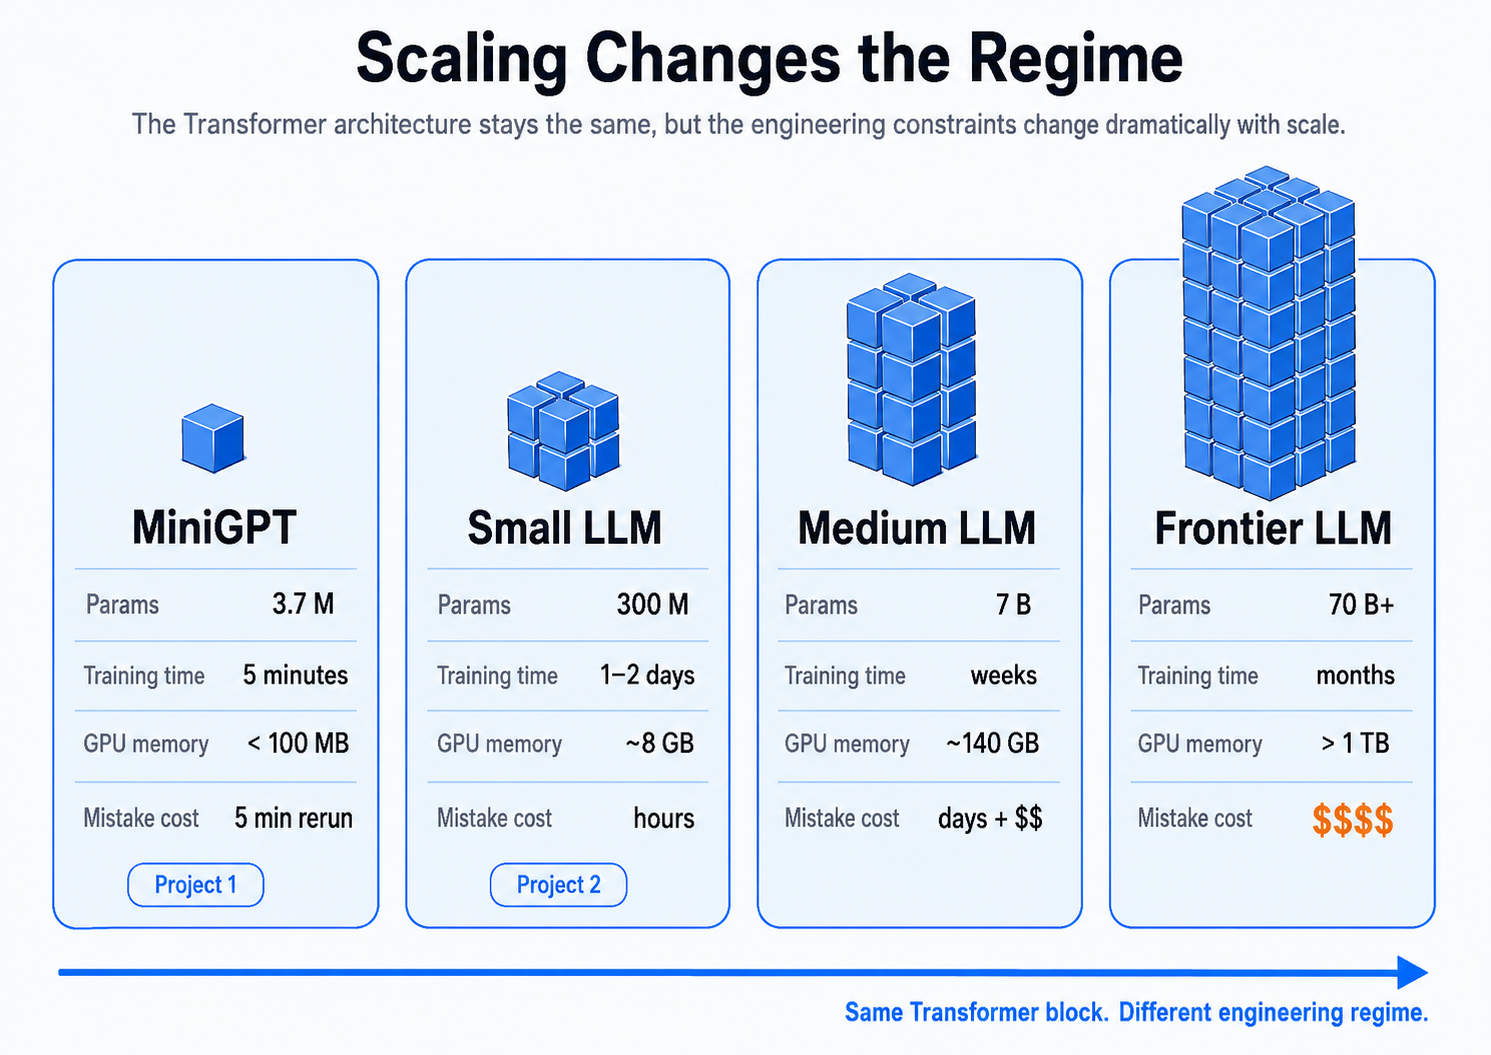
\includegraphics[width=\textwidth]{figures/ch06/fig_scale_gap.png}
  \caption{\textbf{Scaling changes the engineering regime.} The same Transformer block operates in fundamentally different cost structures at different scales. Training time grows from minutes to months; mistake cost grows from a quick rerun to millions of dollars. Project~1 lives in the leftmost column; Project~2 targets the second.}
  \label{fig:scale-gap}
\end{figure}

The qualitative shift is not just ``bigger numbers.'' It is a change in the cost structure of the entire engineering process:

\begin{itemize}[nosep]
  \item \textbf{You cannot iterate by rerunning.} A 7B model that diverges at step~30,000 has already consumed tens of thousands of GPU-hours. ``Just restart'' is not a viable debugging strategy.
  \item \textbf{Memory becomes a first-class constraint.} At 3.7M parameters, memory is invisible. At 7B, the training state does not fit on a single GPU in any precision.
  \item \textbf{Silent failures become expensive failures.} A 5\% quality degradation from a subtle numerical bug costs nothing to discover in Project~1 (compare two five-minute runs). At 7B, you may not discover the bug until the run is complete---weeks later.
  \item \textbf{The data pipeline changes character.} Project~1 loaded 21\,MB into RAM. A 2T-token pretraining run processes $\sim$4\,TB of compressed text through a streaming pipeline that must never repeat, never leak test data, and never stall the GPU.
\end{itemize}

\paragraph{One component update.} Chapter~\ref{ch:decoder-only} introduced Pre-LN---applying LayerNorm before each sub-layer. In practice, most modern LLMs use \textbf{RMSNorm}, a simplification that drops the mean-centering step:
\[
  \text{RMSNorm}(\mathbf{x}) = \frac{\mathbf{x}}{\sqrt{\frac{1}{d}\sum_{i=1}^{d} x_i^2 + \epsilon}} \odot \boldsymbol{\gamma}
\]
The difference from LayerNorm is a single subtraction removed. The practical effect: faster normalization with similar training stability in the regimes where it has become standard. GPT-2 and OPT used LayerNorm; LLaMA-class models moved to RMSNorm. We mention it here because Chapter~\ref{ch:decoder-only} described Pre-LN without specifying the norm variant.

\begin{quickrecap}
\textbf{Quick Recap.}
\begin{itemize}[nosep,leftmargin=1.5em]
  \item Scale changes the cost structure: mistakes go from ``five-minute rerun'' to ``hundred-thousand-dollar loss.''
  \item Memory, stability, data, and debugging all enter new regimes at billions of parameters.
  \item The architecture barely changed since Chapter~\ref{ch:decoder-only}; the engineering around it did.
\end{itemize}
\textit{The first consequence of scale is the simplest: the training state no longer fits in memory.}
\end{quickrecap}


%----------------------------------------------------------------------
\section{The Memory Wall}
\label{sec:memory-wall}

To train a neural network with Adam, the GPU must hold four things simultaneously:

\begin{enumerate}[nosep]
  \item \textbf{Parameters} $\theta$: the model weights.
  \item \textbf{Gradients} $\nabla\theta$: one gradient tensor per parameter.
  \item \textbf{Optimizer states}: Adam maintains a first-moment estimate $m$ and a second-moment estimate $v$ for every parameter---two additional copies.
  \item \textbf{Activations}: the intermediate tensors from the forward pass, kept in memory for the backward pass.
\end{enumerate}

\subsection{Counting Bytes}

Let $N$ be the number of parameters. In fp32 training, each number occupies 4 bytes:

\begin{center}
\begin{tabular}{lll}
\toprule
\textbf{Component} & \textbf{Precision} & \textbf{Per-param bytes} \\
\midrule
Parameters          & fp32              & 4 \\
Gradients           & fp32              & 4 \\
Adam $m$            & fp32              & 4 \\
Adam $v$            & fp32              & 4 \\
\midrule
\textbf{Total (fp32)} &                   & $4+4+4+4 = \mathbf{16}$ \\
\bottomrule
\end{tabular}
\end{center}

In mixed-precision training with bf16, parameters and gradients are stored in half precision during the forward/backward pass, but Adam's states and a master copy of the weights must remain in fp32 for numerical stability:

\begin{center}
\begin{tabular}{lll}
\toprule
\textbf{Component} & \textbf{Precision} & \textbf{Per-param bytes} \\
\midrule
Parameters (master copy)  & fp32   & 4 \\
Parameters (bf16 copy)    & bf16   & 2 \\
Gradients                 & bf16   & 2 \\
Adam $m$                  & fp32   & 4 \\
Adam $v$                  & fp32   & 4 \\
\midrule
\textbf{Total (mixed)} &        & $4+2+2+4+4 = \mathbf{16}$ \\
\bottomrule
\end{tabular}
\end{center}

The total is coincidentally 16 bytes per parameter in both cases: fp32 saves on the extra bf16 copy; mixed precision pays for the bf16 copy but saves on gradient storage.\footnote{The 16-bytes-per-parameter rule assumes AdamW. Alternative optimizers change this number: Lion~\cite{chen2024lion} uses only one momentum buffer (saving $\sim$4$N$ bytes), and Adafactor factorizes the second-moment estimate. The per-parameter cost is a function of optimizer choice, not a physical constant.} The rule of thumb is simple: \textbf{training memory $\approx$ 16$N$ bytes, plus activations.}

\medskip
\noindent\fbox{\parbox{\dimexpr\textwidth-2\fboxsep-2\fboxrule\relax}{\textbf{Pause and verify.} Return to the running example: you want to scale your 3.7M MiniGPT to 7B parameters. Using the 16-bytes-per-parameter rule, compute the training-state memory (excluding activations). Then check: does it fit on a single RTX~4090 (24\,GB)? A single A100~(80\,GB)? Think about this before reading the anchor table below.}}
\medskip

\noindent The answer: $7 \times 10^9 \times 16 = 112$\,GB for training state alone. An RTX~4090 has 24\,GB---you would need nearly five of them just for the static training state, before a single activation is computed. An A100~(80\,GB) falls short by 32\,GB. The 2,000$\times$ increase in parameters produced a 2,000$\times$ increase in memory---but GPU memory did not grow by 2,000$\times$.

\subsection{Activations}

Activations are harder to estimate because they depend on batch size ($B$), context length ($T$), hidden dimension ($d$), and number of layers ($L$). A useful approximation:

\[
  \text{Activation memory} \approx B \times T \times d \times L \times c \text{ bytes}
\]

where $c$ depends on what is stored: the residual stream, QKV projections, the attention output, the FFN's $4d$ intermediate expansion, and (without FlashAttention) the $T \times T$ attention matrices. In practice $c \approx 10$--$30$ for bf16 mixed-precision training; the lower end corresponds to aggressive activation checkpointing (Chapter~\ref{ch:distributed-training}), the upper end to storing everything for fast backward passes.\footnote{Korthikanti et al., ``Reducing Activation Recomputation in Large Transformer Models'' (2023), provide an exact formula for Megatron-LM's activation memory as a function of model configuration and recomputation strategy.} In practice, activations often rival or exceed the parameter-related memory.

\subsection{The Anchor Table}

\begin{center}
\small
\begin{tabular}{lrrrrl}
\toprule
 & \textbf{MiniGPT} & \textbf{300M} & \textbf{7B} & \textbf{70B} & \textbf{Note} \\
\midrule
Parameters        & 3.7M   & 300M   & 7B    & 70B   & \\
Param + Opt (16$N$) & 59\,MB & 4.8\,GB & 112\,GB & 1.1\,TB & \\
Activations (est.)  & tiny   & $\sim$2\,GB & $\sim$30\,GB & $\sim$300\,GB & $B{=}8, T{=}2048$ \\
\midrule
\textbf{Total (est.)} & $<$100\,MB & $\sim$7\,GB & $\sim$140\,GB & $\sim$1.4\,TB & \\
\midrule
RTX 4090 (24\,GB) & \checkmark & tight & \texttimes & \texttimes & \\
A100 (80\,GB) / H100 & \checkmark & \checkmark & tight & \texttimes & \\
H200 (141\,GB)       & \checkmark & \checkmark & \checkmark & \texttimes & \\
B200 (192\,GB)       & \checkmark & \checkmark & \checkmark & \texttimes & \\
B300 (288\,GB)       & \checkmark & \checkmark & \checkmark & \texttimes & \\
\bottomrule
\end{tabular}
\end{center}

The most recent GPUs---NVIDIA's H200 (141\,GB HBM3e), B200 (192\,GB), and B300 (288\,GB HBM3e)---have pushed the single-GPU memory ceiling dramatically. A 7B model's training state ($\sim$140\,GB) fits on an H200 but not on an H100. A 13B model would exceed the H200 but fit on a B300. A 70B model ($\sim$1.4\,TB) exceeds every single GPU by an order of magnitude. Each GPU generation shifts the boundary, but model sizes grow at least as fast.

\begin{figure}[t]
  \centering
  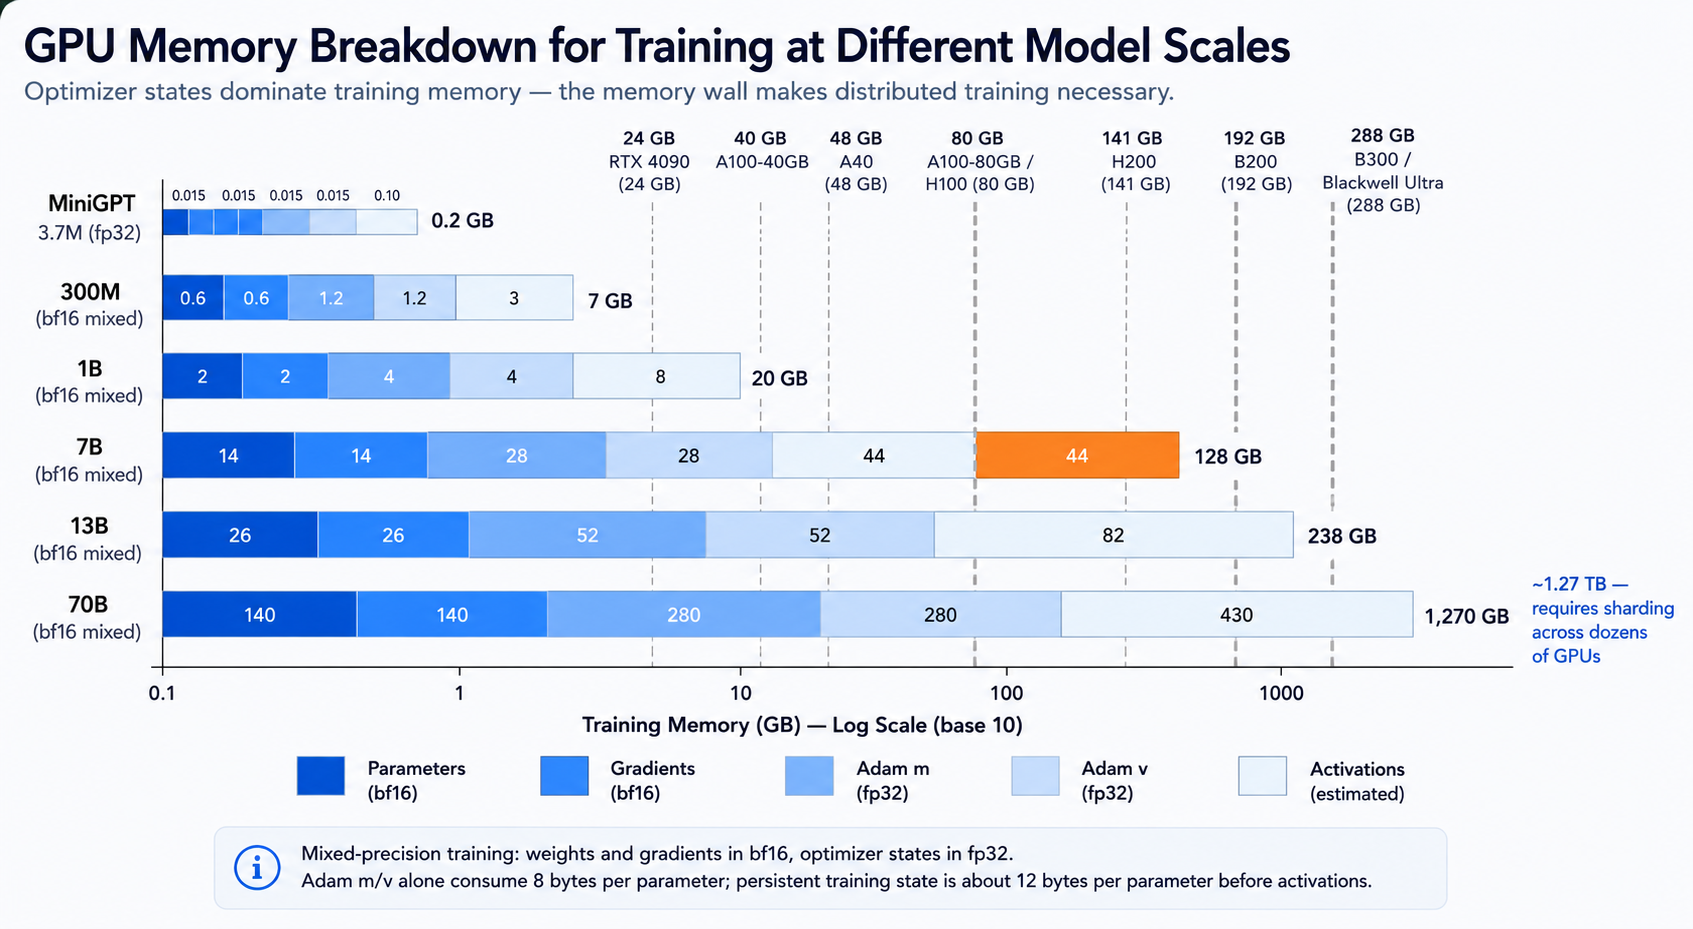
\includegraphics[width=\textwidth]{figures/ch06/fig_memory_wall.png}
  \caption{\textbf{GPU memory breakdown for training at different model scales.} Each bar shows the total training-state memory (parameters, gradients, Adam states, activations) in mixed-precision training. Horizontal lines mark the VRAM of mainstream GPUs from RTX~4090 (24\,GB) to B300 (288\,GB). A 7B model exceeds any single GPU below the H200; a 70B model requires sharding across many devices.}
  \label{fig:memory-wall}
\end{figure}

The anchor table tells a clear story:

\begin{itemize}[nosep]
  \item \textbf{MiniGPT} fits anywhere. Memory is invisible. This is why Project~1 never discussed it.
  \item \textbf{300M} barely fits on a 4090 in bf16. This is the scale of Project~2's baseline.
  \item \textbf{7B} does not fit on any single consumer GPU. Distributed training (Chapter~\ref{ch:distributed-training}) is not an optimization---it is the only way the training state fits.
  \item \textbf{70B} requires hundreds of gigabytes of aggregate memory. Even a multi-GPU setup must carefully shard parameters, gradients, and optimizer states across devices.
\end{itemize}

\begin{quickrecap}
\textbf{Quick Recap.}
\begin{itemize}[nosep,leftmargin=1.5em]
  \item Training memory $\approx$ 16 bytes per parameter (params + grads + Adam states), plus activations.
  \item A 7B model needs $\sim$140\,GB just for training state---more than any single GPU.
  \item Distributed training is not a performance optimization; it is a memory necessity.
\end{itemize}
\textit{Memory pressure explains why we need multiple GPUs. But even on a single GPU, there is another bottleneck: the attention computation itself.}
\end{quickrecap}


%----------------------------------------------------------------------
\section{FlashAttention: Same Math, Different Memory Access}
\label{sec:flash-attention}

The memory wall tells you that the 7B model's \emph{static} training state does not fit on one GPU. But there is a second memory problem---one that is hidden inside a formula you already know.

Chapter~\ref{ch:attention} derived the attention formula:
\[
  \text{Attention}(Q, K, V) = \text{softmax}\!\left(\frac{QK^\top}{\sqrt{d_k}}\right) V
\]
At context length $T$, the intermediate matrix $QK^\top$ has shape $T \times T$. For Project~1's $T = 256$, this matrix has 65,536 entries per head per batch element---a rounding error on any modern GPU. But at $T = 4096$ (typical for LLaMA-class models), it has 16.7 million entries. At $T = 32{,}768$ (GPT-4 class), it has over one billion entries.

The standard implementation computes attention in three steps:

\begin{enumerate}[nosep]
  \item Compute $S = QK^\top / \sqrt{d_k}$ --- read $Q, K$ from GPU main memory (HBM), write $S$ back to HBM.
  \item Compute $P = \text{softmax}(S)$ --- read $S$ from HBM, write $P$ back to HBM.
  \item Compute $O = PV$ --- read $P, V$ from HBM, write $O$ back to HBM.
\end{enumerate}

Each step performs a round-trip to HBM (High Bandwidth Memory)---the GPU's main memory, which is large ($\sim$80\,GB on an A100) but slow relative to the GPU's on-chip SRAM ($\sim$20\,MB, but 10--20$\times$ faster). The total HBM traffic scales as $O(T^2)$ because the $T \times T$ matrices $S$ and $P$ must be written and read back.

\paragraph{The key insight.} On modern GPUs, the attention computation at long context lengths is not limited by arithmetic---the GPU has more than enough floating-point throughput. It is limited by \textbf{memory bandwidth}: the time spent moving the $T \times T$ attention matrix between HBM and the compute units. This is the IO bottleneck.

\paragraph{A concrete example.} Return to the running example. Your MiniGPT uses $T = 256$ and $h = 4$ heads. The attention matrix per head per batch element is $256 \times 256 = 65{,}536$ entries $\times$ 2 bytes (bf16) = 128\,KB. With batch size 32, all heads together: $4 \times 32 \times 128\,\text{KB} = 16\,$MB. Negligible.

Now scale to the 7B model: $T = 4096$, $h = 32$ heads, $B = 8$. The attention matrix per head per batch element is $4096 \times 4096 = 16.8$M entries $\times$ 2 bytes = 33.6\,MB. Across all heads and batch elements: $32 \times 8 \times 33.6\,\text{MB} \approx 8.6\,$GB---\emph{just for intermediate attention matrices}. This is memory that exists only during the forward pass, holds no learned information, and is thrown away after softmax. At $T = 32{,}768$ the number exceeds 500\,GB. The attention formula did not change. The numbers did.

\subsection{The FlashAttention Approach}

FlashAttention~\cite{dao2022flashattention} eliminates the IO bottleneck by never materializing the full $T \times T$ attention matrix in HBM. The core idea:

\begin{enumerate}[nosep]
  \item \textbf{Tile the computation.} Divide $Q$, $K$, $V$ into small blocks that fit in on-chip SRAM.
  \item \textbf{Compute attention within SRAM.} For each block of queries, load the corresponding blocks of keys and values into SRAM, compute the local attention scores, and accumulate the output---all without writing intermediate results to HBM.
  \item \textbf{Use online softmax.} Standard softmax requires a full pass over all scores to compute the normalization constant. FlashAttention uses an \emph{online} algorithm that updates the running softmax statistics as each key block is processed, producing the exact same result as the standard formula.
\end{enumerate}

The result: the full $T \times T$ matrix never exists in HBM. Only the final output $O$ (shape $T \times d$, not $T \times T$) is written back. HBM traffic drops from $O(T^2)$ to $O(T)$ in the sequence length dimension.

\begin{figure}[t]
  \centering
  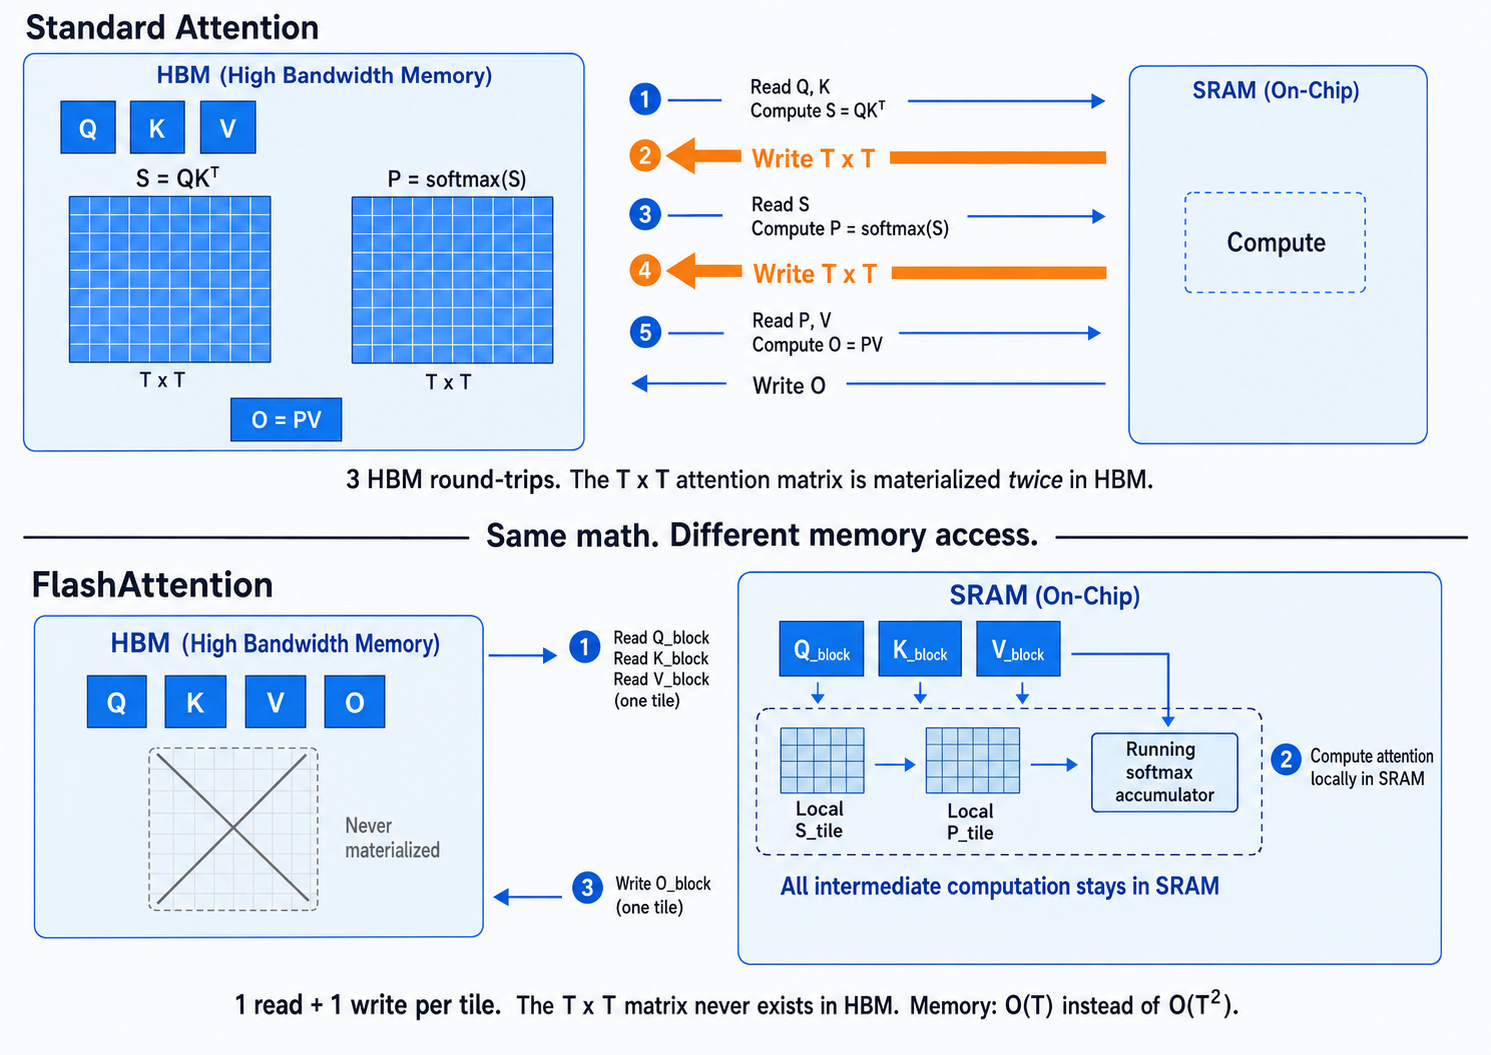
\includegraphics[width=\textwidth]{figures/ch06/fig_flash_attention.png}
  \caption{\textbf{Standard attention vs.\ FlashAttention.} \textbf{Top:} standard attention performs three HBM round-trips, materializing the full $T \times T$ score and probability matrices. \textbf{Bottom:} FlashAttention tiles $Q$, $K$, $V$ into blocks that fit in on-chip SRAM, computes attention within SRAM using online softmax, and writes only the final output to HBM. The $T \times T$ matrix never exists in main memory.}
  \label{fig:flash-attention}
\end{figure}

\subsection{What Changes and What Doesn't}

\begin{center}
\begin{tabular}{lcc}
\toprule
 & \textbf{Standard} & \textbf{FlashAttention} \\
\midrule
Mathematical result        & exact & mathematically equivalent \\
HBM reads/writes           & $O(T^2 d)$ & $O(T^2 d^2 / M)$\textsuperscript{*} \\
Peak HBM usage             & $O(T^2)$ per head & $O(T)$ per head \\
Wall-clock speed            & 1$\times$ & 2--4$\times$ faster \\
Causal masking support      & yes & yes (fused) \\
Backpropagation support     & yes & yes (recomputation) \\
\bottomrule
\end{tabular}
\end{center}

\noindent\textsuperscript{*}$M$ is the SRAM size. The IO complexity is subquadratic in $T$ for typical values.

\medskip

The critical point: \textbf{FlashAttention does not approximate attention.} It computes the same attention function as the standard formula, up to normal floating-point differences from a different accumulation order. The improvement is purely in how data moves between memory levels---it is a systems optimization, not an algorithmic change.

\medskip
\noindent\fbox{\parbox{\dimexpr\textwidth-2\fboxsep-2\fboxrule\relax}{\textbf{Pause and verify.} An A100 GPU has $\sim$2\,TB/s of HBM bandwidth and $\sim$20\,MB of SRAM. For the 7B model at $T = 4096$, the standard attention writes $\sim$8.6\,GB of intermediate matrices to HBM per forward pass. How long does just the \emph{writing} take at 2\,TB/s? Now consider: a single forward-backward step also reads those matrices back. FlashAttention avoids both trips. Where does that time go instead?}}
\medskip

\paragraph{Why Project~1 didn't need it.} At $T = 256$, the attention matrix is tiny (128\,KB per head in bf16). HBM bandwidth is not the bottleneck---compute is. FlashAttention provides no meaningful speedup at short context lengths on small models. The benefits emerge at $T \geq 1024$ and become dramatic at $T \geq 4096$.

\paragraph{Why production needs it.} At $T = 4096$ with 32 heads and batch size 8, the standard attention matrices consume $\sim$16\,GB of HBM just for intermediates. FlashAttention reduces this to near zero. Without it, long-context training at scale would require either (a) far more GPUs or (b) far shorter context windows. FlashAttention is the single engineering contribution that made long-context LLMs practical.

\begin{quickrecap}
\textbf{Quick Recap.}
\begin{itemize}[nosep,leftmargin=1.5em]
  \item Standard attention materializes a $T \times T$ matrix in GPU main memory---the IO bottleneck.
  \item FlashAttention tiles the computation into SRAM, uses online softmax, and never writes the full attention matrix to HBM.
  \item The mathematical result is identical. The memory usage drops from $O(T^2)$ to $O(T)$.
  \item FlashAttention doesn't matter at $T = 256$ (Project~1). It is essential at $T \geq 4096$ (production LLMs).
\end{itemize}
\textit{Memory and IO are now under control. But scale introduces a third kind of problem: failures that take hours or days to manifest.}
\end{quickrecap}


%----------------------------------------------------------------------
\section{Stability Failures at Scale}
\label{sec:scale-stability}

Chapter~\ref{ch:tokens-to-training} cataloged failure modes for small models: NaN from too-high learning rate, unshifted labels, missing warmup. These failures are \emph{loud}---they manifest within the first hundred steps, and a five-minute rerun confirms the fix.

At scale, a different class of failures emerges. Think of the difference between a car that won't start (loud failure---you know immediately) and a car with a slow oil leak (silent failure---everything seems fine until the engine seizes on the highway, a hundred miles from home). The loud failures are cheap: you pop the hood, find the loose wire, restart. The silent failures are catastrophic: by the time you notice, you have already lost something you cannot easily recover. Scale turns loud failures into silent ones---and silent ones into expensive ones.

\subsection{Loss Spikes}

A loss spike is a sudden, sharp increase in the training loss after thousands of stable steps. The loss may recover on its own, or it may settle at a permanently higher plateau. In either case, the compute spent during and after the spike is partially or fully wasted.

Loss spikes at scale have several known causes:

\begin{itemize}[nosep]
  \item \textbf{Bad batches.} A single batch with anomalous content (extremely long sequences, corrupted text, or degenerate patterns) can produce an outlier gradient that destabilizes the model. Gradient clipping mitigates this but does not eliminate it.
  \item \textbf{Numerical accumulation errors.} In bf16 training, gradient accumulation over many micro-batches can drift if intermediate sums are not computed in fp32. A small per-step error compounds over thousands of steps.
  \item \textbf{Learning rate schedule interactions.} If the learning rate is still relatively high when the model encounters a sudden distribution shift in the data (e.g., switching from web text to code), the optimizer may overshoot.
\end{itemize}

The OPT-175B training logbook~\cite{zhang2022opt}, publicly released by Meta, documents dozens of loss spikes, manual interventions, and restarts across months of training. It remains one of the most valuable case studies in large-scale training engineering---not because OPT was the best model, but because the team documented every failure in real time.

\subsection{Attention Logit Growth}

In deep Transformers, the dot-product attention scores $QK^\top / \sqrt{d_k}$ can grow in magnitude over the course of training. When scores become very large, the softmax output concentrates on a single token---attention entropy collapses. This is a slow, insidious failure: the loss may continue to decrease, but the model's ability to attend to diverse context positions degrades.

Mitigation strategies include:
\begin{itemize}[nosep]
  \item \textbf{QK-norm:} applying RMSNorm to queries and keys before the dot product, bounding the score magnitudes.
  \item \textbf{Logit capping:} clamping attention logits to a fixed range (e.g., $[-50, 50]$) before softmax.
  \item \textbf{z-loss:} adding an auxiliary penalty on the log-partition function of the softmax, regularizing the scale of logits throughout training. Used in PaLM~\cite{chowdhery2023palm} and subsequent models.
  \item \textbf{Careful initialization:} scaling the query and key projections so that initial attention scores have unit variance.
\end{itemize}

\subsection{Silent Quality Degradation}

The most dangerous failures at scale are the ones where \emph{nothing looks wrong}. The loss decreases smoothly. The gradient norms are stable. The throughput is nominal. But the final model is 5--10\% worse than it should be on downstream benchmarks.

Common causes:
\begin{itemize}[nosep]
  \item \textbf{Data contamination.} Training data overlaps with evaluation benchmarks. The loss looks excellent; the benchmark scores are inflated; the model has not actually learned the capability being tested.
  \item \textbf{Precision drift.} bf16 arithmetic introduces small rounding errors that, over millions of steps, systematically bias certain weight distributions. The effect is invisible in the loss curve but measurable in generation quality.
  \item \textbf{Distributed training bugs.} One GPU in a multi-node setup computes slightly different gradients due to a software version mismatch or hardware fault. The averaged gradient is subtly wrong, and the model trains on corrupted signal without any visible error. At frontier scale, \emph{silent data corruptions} (SDCs)---bit-flips in GPU memory or arithmetic units that produce wrong-but-plausible results---are a documented engineering reality~\cite{dixit2021silent}.
\end{itemize}

\begin{figure}[t]
  \centering
  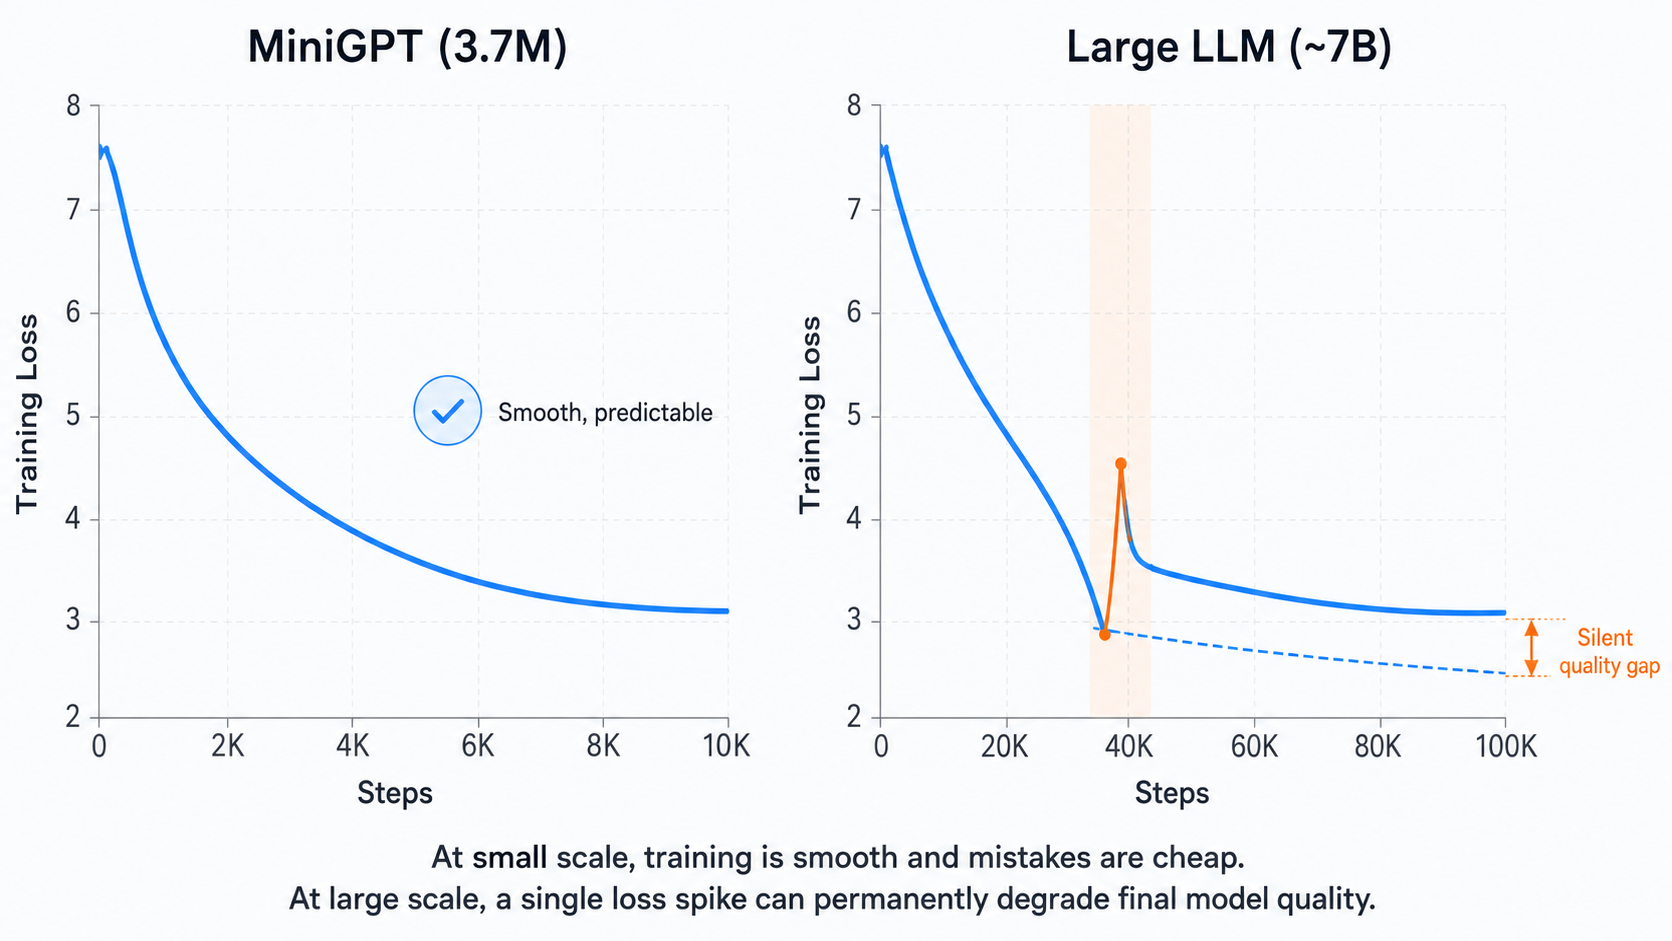
\includegraphics[width=\textwidth]{figures/ch06/fig_loss_spike.png}
  \caption{\textbf{Stability at small vs.\ large scale.} \textbf{Left:} MiniGPT (3.7M) training is smooth and predictable---mistakes are discovered in minutes. \textbf{Right:} a large model ($\sim$7B) may train stably for tens of thousands of steps before a loss spike occurs. Even after recovery, the model may settle at a worse trajectory (silent quality gap). Adapted from the failure patterns documented in the OPT-175B training logbook~\cite{zhang2022opt}.}
  \label{fig:loss-spike}
\end{figure}

\paragraph{What to watch.} In Project~1, you diagnosed problems by comparing two five-minute runs. At scale, you cannot afford reference runs. Instead, industrial training relies on \emph{monitoring infrastructure}---dashboards that track multiple signals in real time. The key diagnostic channels:

\begin{center}
\small
\begin{tabularx}{\textwidth}{@{}lXl@{}}
\toprule
\textbf{Signal} & \textbf{What it tells you} & \textbf{Red flag} \\
\midrule
Training loss & Overall learning progress & Sudden spike $>2\times$ baseline \\
Gradient norm & Optimization stability & Sustained increase over 1K steps \\
Activation scale & Layer health & Max activation $> 10^4$ \\
Learning rate & Schedule correctness & Unexpected jump after resume \\
Tokens/sec & Hardware utilization & Drop $> 10\%$ from baseline \\
Val loss vs.\ train loss & Overfitting / data issues & Gap widens steadily \\
\bottomrule
\end{tabularx}
\end{center}

Chapter~\ref{ch:distributed-training} will cover the engineering of this monitoring in the context of distributed training.

\begin{quickrecap}
\textbf{Quick Recap.}
\begin{itemize}[nosep,leftmargin=1.5em]
  \item Scale introduces \emph{silent} failures: loss spikes after thousands of stable steps, attention-logit growth, and precision drift.
  \item The most dangerous failures are the ones where nothing looks wrong---the model trains smoothly but ends up worse than expected.
  \item Diagnosis at scale requires monitoring infrastructure, not rerunning.
\end{itemize}
\textit{Failures are expensive. This changes not just the debugging process but the entire engineering workflow.}
\end{quickrecap}


%----------------------------------------------------------------------
\section{The Pilot Run Discipline}
\label{sec:pilot-runs}

In Project~1, the workflow was simple: write code, run training, check results, fix bugs, repeat. You ran Ablation~4 (five learning rates $\times$ 10K steps each) in under an hour. The cost of being wrong was five minutes of GPU time.

Now return to the running example. Your 7B model takes weeks per run. Running five learning rates is not an afternoon experiment---it is a month of compute. You cannot afford to discover at step~50,000 that your learning rate is 2$\times$ too high. The entire engineering workflow must change.

Industrial pretraining teams solve this with a staged workflow:

\begin{enumerate}[nosep]
  \item \textbf{Tiny smoke run} ($\sim$100 steps, smallest model). Verifies that the code runs end-to-end without errors. Catches data pipeline bugs, shape mismatches, and configuration mistakes. Takes minutes.
  \item \textbf{Small recipe pilot} ($\sim$1K steps, 1/10 scale). Verifies that the training recipe produces a reasonable loss curve shape. Catches learning rate, warmup, and initialization problems. Takes hours.
  \item \textbf{Medium scaling pilot} ($\sim$5K--10K steps, 1/3 scale). Verifies that the loss trajectory is on track for the target final loss. If you have scaling-law estimates (Chapter~\ref{ch:scaling-laws}), this run validates that your configuration is in the right ballpark. Takes a day.
  \item \textbf{Final run} (full scale, full budget). Commits the remaining compute. By this point, the recipe has been validated at three smaller scales. Surprises still happen, but the probability of a catastrophic configuration error is low.
\end{enumerate}

\begin{figure}[t]
  \centering
  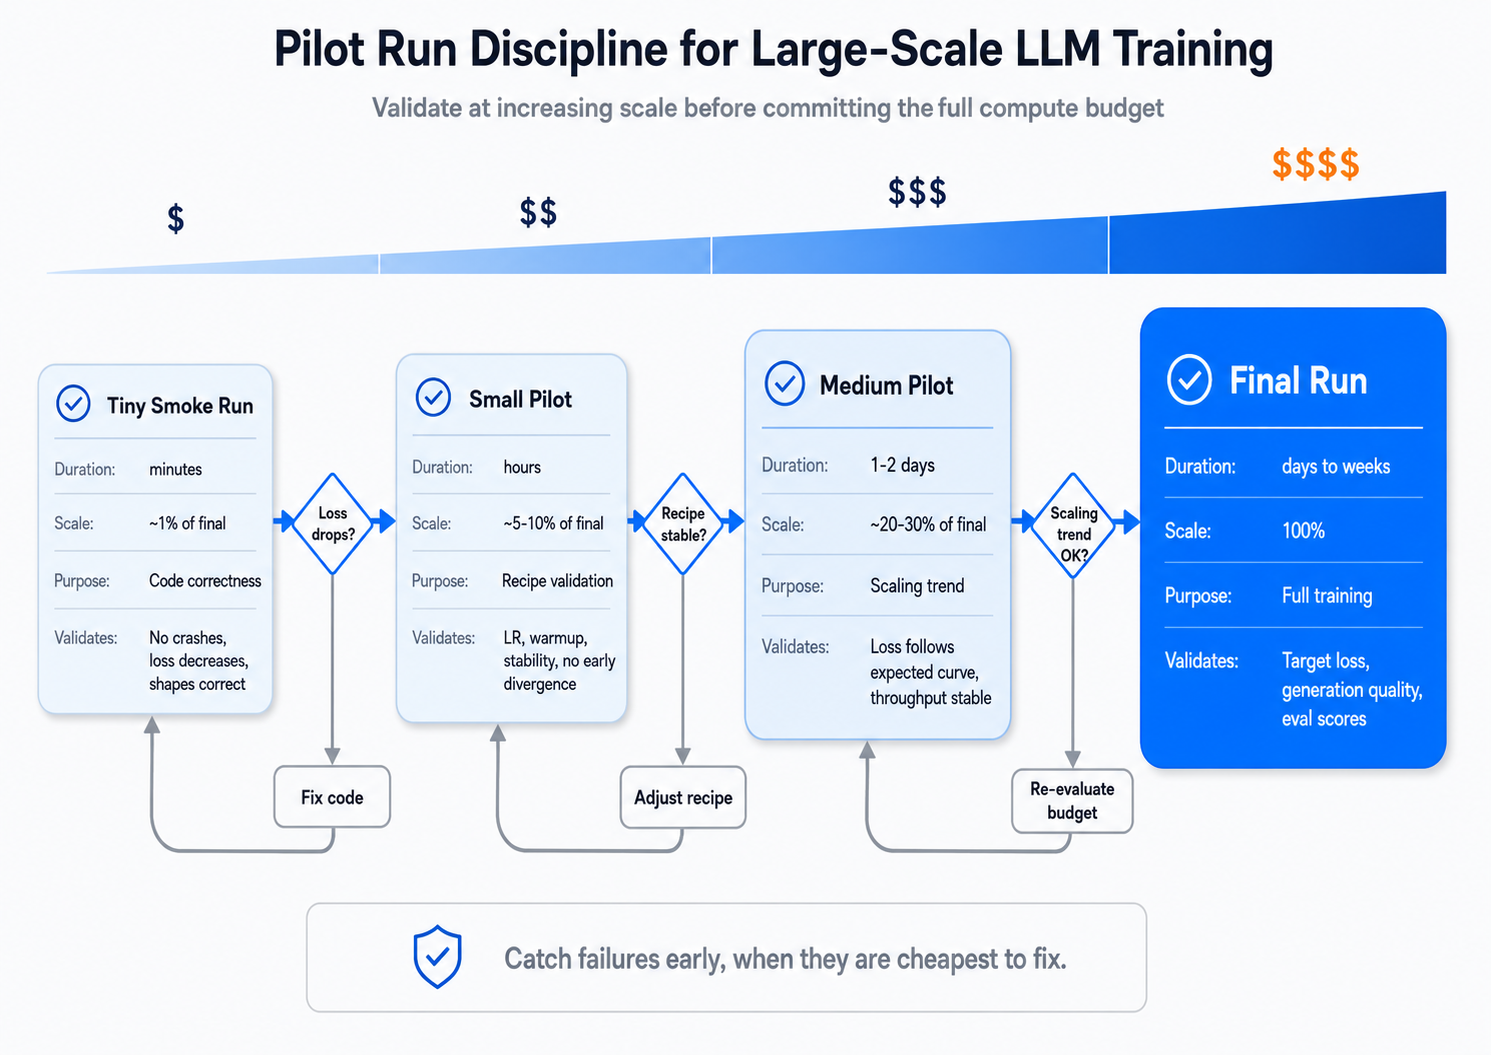
\includegraphics[width=\textwidth]{figures/ch06/fig_pilot_workflow.png}
  \caption{\textbf{The pilot run discipline.} Industrial pretraining validates recipes at increasing scale before committing the full compute budget. Each stage has a specific purpose and a gate condition for proceeding. The total pilot cost (5--10\% of budget) is a small insurance premium against catastrophic configuration errors in the final run.}
  \label{fig:pilot-workflow}
\end{figure}

The pilot methodology is not optional at scale---it is the primary risk-mitigation tool. The total compute spent on pilots is typically 5--10\% of the final run's budget, a small insurance premium against wasting the other 90\%.

\paragraph{This is documented practice, not folklore.} Chinchilla~\cite{hoffmann2022training} is the textbook example: Hoffmann et al.\ trained over 400 models at scales from 70M to 16B parameters, fitting scaling-law curves to small runs before committing the compute for the final 70B model. The LLaMA-3 training report describes a similar staged process---validating learning rate, batch size, and data mix at 1/10 scale before launching the 405B final run. ByteDance's MegaScale paper documents the same discipline at 10,000-GPU scale, including automated pilot-run pipelines that flag anomalous loss curves before human review.

\subsection{Parameter Coupling}

Chapter~\ref{ch:tokens-to-training} introduced training hyperparameters individually: learning rate, batch size, warmup steps, gradient clipping. At small scale, these parameters are largely independent---you can tune them one at a time. At scale, they are \textbf{coupled}, and changing one requires adjusting others:

\begin{itemize}[nosep]
  \item \textbf{Batch size $\leftrightarrow$ learning rate.} The linear scaling rule~\cite{goyal2017imagenet}: if you double the batch size, double the learning rate. The intuition is that larger batches produce lower-variance gradient estimates, so you can take larger steps. This rule holds in the small-to-medium batch regime; beyond the \emph{critical batch size}~\cite{mccandlish2018empirical}, gradient noise is already negligible and further scaling yields diminishing returns---$\sqrt{}$-scaling is closer to optimal. Violating this coupling causes either underfitting (batch doubled, LR unchanged) or instability (LR doubled, batch unchanged).
  \item \textbf{Gradient accumulation $\leftrightarrow$ communication overhead.} In distributed training, each gradient synchronization step incurs communication cost (AllReduce operations across GPUs; Chapter~\ref{ch:distributed-training} covers the mechanics). More accumulation steps mean fewer synchronizations, higher throughput, but larger effective batch size---which circles back to the LR coupling above.
  \item \textbf{Context length $\leftrightarrow$ activation memory.} Doubling the context length roughly doubles activation memory (and quadruples the naive attention cost, though FlashAttention reduces this). A longer context may improve model quality but requires either fewer layers, a smaller batch, or gradient checkpointing (Chapter~\ref{ch:distributed-training}) to fit in memory.
  \item \textbf{Checkpoint cadence $\leftrightarrow$ recovery cost.} More frequent checkpoints waste IO bandwidth and storage but reduce the amount of compute lost when a failure occurs. The optimal cadence depends on the expected failure rate---which itself depends on hardware reliability, cluster size, and training duration.
  \item \textbf{Model size $\leftrightarrow$ data requirement.} Scaling laws (Chapter~\ref{ch:scaling-laws}) show that larger models need proportionally more data to reach their potential. Choosing a model size implicitly commits you to a token budget---and a data pipeline capable of delivering it.
\end{itemize}

\medskip
\noindent\fbox{\parbox{\dimexpr\textwidth-2\fboxsep-2\fboxrule\relax}{\textbf{Pause and verify.} In Project~1, you found that \texttt{lr=3e-3} worked better than the default \texttt{lr=3e-4} (Ablation~4). Suppose you now quadruple the batch size for the 7B model. According to the linear scaling rule, what should the new learning rate be? And if you also switch from $T=256$ to $T=4096$, how does that change the activation memory? Trace the coupling chain: one change in batch size cascades into LR, communication cost, and memory pressure.}}
\medskip

\paragraph{The recipe as a system.} A training recipe is not a list of independently tuned hyperparameters. It is a \emph{system} in which every parameter constrains every other. This is why industrial teams validate recipes at small scale before committing large compute: changing one parameter at full scale and discovering it breaks the coupling is catastrophically expensive.

\paragraph{A partial solution: $\mu$P.} The Maximal Update Parametrization ($\mu$P)~\cite{yang2022tensor} proposes a principled initialization and learning-rate scaling scheme under which hyperparameters tuned on a small model \emph{transfer directly} to a larger model with the same architecture. If $\mu$P holds, the small-scale pilot becomes a true proxy for the final run, not just a plausibility check. In practice, $\mu$P transfer is imperfect---it works best for width scaling and less reliably across depth or architectural changes---but many frontier teams use it as a starting point for their pilot methodology.

\begin{quickrecap}
\textbf{Quick Recap.}
\begin{itemize}[nosep,leftmargin=1.5em]
  \item Industrial pretraining uses staged pilot runs: tiny smoke $\to$ small pilot $\to$ medium pilot $\to$ final run.
  \item Pilot runs cost 5--10\% of the total budget but prevent catastrophic configuration errors.
  \item Training parameters are coupled at scale: batch--LR, context--memory, checkpoint--recovery, model--data.
  \item A recipe is a system of interdependent parameters, not a list of independent choices.
\end{itemize}
\textit{This chapter has traced a chain: scale creates memory pressure, IO bottlenecks, stability risks, and cost constraints that together demand a new engineering discipline. The remaining chapters of Part~II address each link in this chain.}
\end{quickrecap}


%----------------------------------------------------------------------
\section{Beyond the Dense Stack}
\label{sec:frontier-variants}

This chapter assumed a dense decoder-only Transformer---every parameter is active for every token. But two architectural departures have become central to frontier models since 2023:

\begin{itemize}[nosep]
  \item \textbf{Mixture-of-Experts (MoE).} Instead of one large FFN per layer, MoE models maintain $E$ expert FFNs and a learned router that activates only $k \ll E$ experts per token. A model with 400B total parameters might activate only 50B per token, achieving the quality of a dense 400B model at the inference cost of a 50B model. MoE reshapes every axis of the scaling problem: memory (total parameters are large, but active parameters are small), communication (expert routing introduces all-to-all traffic patterns distinct from standard AllReduce), and stability (router collapse and load imbalance are new failure modes). Mixtral~\cite{jiang2024mixtral}, DeepSeek-V3, and reportedly GPT-4 all use MoE routing.
  \item \textbf{Inference-time compute scaling.} Models like OpenAI's o1/o3 and DeepSeek-R1 scale compute at \emph{inference} time rather than (only) at training time---generating long chains of reasoning tokens before producing a final answer. This shifts the scaling equation: instead of ``bigger model $=$ better,'' it becomes ``more thinking time $=$ better on hard problems.'' The training pipeline changes too: these models require reinforcement learning or search-based fine-tuning, which is the territory of Part~III.
\end{itemize}

We do not cover MoE or inference-time scaling in depth in this chapter---the dense GPT stack is the foundation, and Project~2 targets dense models. But a PhD-level understanding of scaling must include the awareness that ``making the model bigger'' is no longer the only axis of improvement.


%----------------------------------------------------------------------
\section{Part II Roadmap}
\label{sec:part2-roadmap}

Each chapter in Part~II solves a specific problem that this chapter identified:

\begin{center}
\small
\begin{tabularx}{\textwidth}{@{}p{0.23\textwidth}p{0.34\textwidth}X@{}}
\toprule
\textbf{Chapter} & \textbf{Problem} & \textbf{Key question} \\
\midrule
Ch.~\ref{ch:distributed-training}: Distributed Training &
  The training state does not fit on one GPU. &
  How do you shard parameters, gradients, and optimizer states across devices? \\[4pt]
Ch.~\ref{ch:scaling-laws}: Scaling Laws &
  Compute is finite. &
  Given a fixed GPU budget, what model size and token count produce the best model? \\[4pt]
Ch.~\ref{ch:data-engineering}: Data Engineering &
  More tokens are needed than any single source provides. &
  How do you collect, filter, deduplicate, and mix trillions of tokens of training data? \\[4pt]
Ch.~\ref{ch:evaluation}: Evaluation &
  Loss alone does not tell you if the model is good. &
  How do you measure what a language model can and cannot do? \\
\bottomrule
\end{tabularx}
\end{center}

\textbf{Project~2} sits after all five chapters. It requires students to make and justify data, scaling, distributed-training, and evaluation decisions under a fixed compute budget (4$\times$H100, limited GPU-hours)---turning the concepts of Part~II into engineering practice, just as Project~1 did for Part~I.

\medskip
\noindent Beyond Part~II, Part~III takes the pretrained model and asks: \emph{how do you make it useful and aligned?} Instruction tuning, RLHF, and inference-time reasoning---the topics that turned base language models into the tools people actually use---begin there.


%----------------------------------------------------------------------

\begin{takeaways}
\begin{itemize}[leftmargin=1.2em, itemsep=4pt]
  \item Scaling does not just make the model bigger. It changes the memory regime, the IO profile, the stability landscape, the cost of mistakes, and the engineering workflow.
  \item \textbf{Training memory} $\approx$ 16 bytes per parameter (params + grads + Adam states), plus activations. A 7B model needs $\sim$140\,GB---more than any single GPU.
  \item \textbf{FlashAttention} computes the exact same attention output but avoids materializing the $T \times T$ matrix in HBM, reducing memory from $O(T^2)$ to $O(T)$. It is a systems optimization, not an algorithmic change.
  \item Scale-specific failures are \textbf{silent}: loss spikes after long stable training, attention-logit growth, precision drift, and data contamination. The most dangerous failures are the ones where nothing looks wrong.
  \item Industrial pretraining uses \textbf{pilot runs} at 1/10 scale to validate recipes before committing the full compute budget. Training parameters are coupled (batch--LR, context--memory, model--data), so a recipe is a system, not a list.
  \item Part~II addresses each scaling problem in turn: distributed training (Ch.~\ref{ch:distributed-training}), scaling laws (Ch.~\ref{ch:scaling-laws}), data engineering (Ch.~\ref{ch:data-engineering}), and evaluation (Ch.~\ref{ch:evaluation}).
\end{itemize}
\end{takeaways}


%----------------------------------------------------------------------
\section{Summary}

\paragraph{What this chapter established.} Part~I taught you to build a correct training system. This chapter showed why correctness is necessary but not sufficient: at scale, memory constraints, IO bottlenecks, stability risks, and cost structures create an entirely different engineering regime. The same architecture that trains in five minutes at 3.7M parameters becomes a months-long, million-dollar endeavor at 70B.

\paragraph{The causal chain.} Scale creates memory pressure (the training state exceeds any single GPU) $\to$ memory pressure exposes IO bottlenecks (attention becomes bandwidth-limited, solved by FlashAttention) $\to$ longer runs surface silent failure modes (loss spikes, precision drift, attention collapse) $\to$ silent failures are expensive (rerunning is not viable) $\to$ expensive failures demand engineering discipline (pilot runs, parameter coupling, monitoring).

\paragraph{One sentence.} The dense Transformer block barely changed since 2017. What changed was the engineering regime around it---plus two architectural departures (MoE, inference-time compute) that Part~II and Part~III will address.


%----------------------------------------------------------------------
\section*{Key Equations at a Glance}

\begin{center}
\begin{tabularx}{\textwidth}{@{}p{4cm}X@{}}
\toprule
\textbf{Quantity} & \textbf{Expression} \\
\midrule
Training memory (per param) & 16 bytes (fp32 or mixed bf16) \\
Total training state & $16N + \text{activations}$ \\
Activation estimate & $\sim B \times T \times d \times L \times c$ bytes, $c \approx 10$--$30$ \\
RMSNorm & $\text{RMSNorm}(\mathbf{x}) = \frac{\mathbf{x}}{\sqrt{\frac{1}{d}\sum x_i^2 + \epsilon}} \odot \boldsymbol{\gamma}$ \\
Attention HBM (standard) & $O(T^2 d)$ per head \\
Attention HBM (Flash) & $O(T^2 d^2 / M)$, peak $O(T)$ per head \\
\bottomrule
\end{tabularx}
\end{center}


%----------------------------------------------------------------------
\section*{Key Readings}

\begin{enumerate}[nosep]
  \item \textbf{Dao et al., 2022.} \textit{FlashAttention: Fast and Memory-Efficient Exact Attention with IO-Awareness.}~\cite{dao2022flashattention} The paper that made long-context training practical. Focus on Section~2 (IO complexity analysis) and Section~3 (the tiling algorithm).
  \item \textbf{Zhang et al., 2022.} \textit{OPT: Open Pre-trained Transformer Language Models.}~\cite{zhang2022opt} The appendix contains a detailed training logbook documenting loss spikes, restarts, and manual interventions during 175B-parameter training. The most honest public account of large-scale training difficulties.
  \item \textbf{Touvron et al., 2023.} \textit{LLaMA: Open and Efficient Foundation Language Models.}~\cite{touvron2023llama} The training recipe section demonstrates the modern LLM stack in practice: RMSNorm, SwiGLU, RoPE, cosine schedule, and the pilot-run approach to large-scale training.
  \item \textbf{Yang et al., 2022.} \textit{Tensor Programs V: Tuning Large Neural Networks via Zero-Shot Hyperparameter Transfer.}~\cite{yang2022tensor} The $\mu$P framework for transferring hyperparameters from small to large models. Relevant to \S\ref{sec:pilot-runs}.
  \item \textbf{Jiang et al., 2024.} \textit{Mixtral of Experts.}~\cite{jiang2024mixtral} A concrete example of MoE at scale: 8$\times$7B experts with top-2 routing, achieving dense-13B quality at 7B inference cost.
\end{enumerate}
